\section{绝热式固定床反应器}


\begin{frame}
    \frametitle{绝热反应器的类型}

    \begin{itemize}
        \item 单段固定床绝热反应器
            \begin{itemize}
                \item[\bigcirc ] 结构简单，空间利用率高，造价低。
                \item[\times ] 对于一些热效应大的反应，反应器出口温度可能会超过允许的温度。
                \item[\times ] 由于温升过大，对于可逆放热反应，反应器的轴向温度分布会远离最佳温度分布，从而造成反应器的生产能力降低。
                \item 适用于反应热效应较小的反应；
                \item 温度对目的产物收率影响不大的反应；
                \item 反应热效应大，但温升小的反应。
            \end{itemize}
        
        \item 多段固定床绝热反应器
            \begin{itemize}
                \item 间接换热式
                \item 原料气冷激式
                \item 非原料气冷激式
            \end{itemize}
        
    \end{itemize}

\end{frame}


\begin{frame}
    \frametitle{间接换热式}

        \begin{minipage}{0.71\linewidth}
            \begin{enumerate}
                \item 原料气经第1、2、3、4换热器预热后，进入第I段反应。
                \item 第I段出来的物料，经4换热后进入第II段反应。
                \item 第II段出来的物料，经3换热后进入第III段反应。
                \item 第III段出来的物料，经2换热后进入第IV段反应。
                \item 产品经预热器1回收热量，送入下一工序。 
            \end{enumerate}
            \bigskip
            \begin{itemize}
                \item 冷却介质是原料气
                \item 反应与换热交替进行
            \end{itemize}
        \end{minipage}\hfill
        \begin{minipage}{0.28\linewidth}
            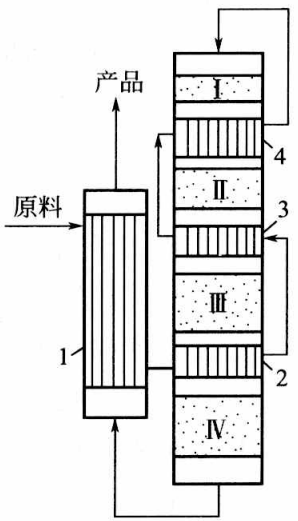
\includegraphics[width=\linewidth]{figures/fig7.3a.png}
        \end{minipage}

\end{frame}


\begin{frame}
    \frametitle{原料气冷激式}

        \begin{minipage}{0.65\linewidth}
            \begin{itemize}
                \item 利用补加冷物料的方法使反应后的物料温度降低，所用的冷激剂为冷原料气。
                \item 原料气只有一部分经预热器1预热至反应温度，其余部分冷的原料气则作冷激用。
                \item 经预热的原料气进入第I段反应，反应后的气体与冷原料气相混合而使其温度降低，再进入第II段反应，依次类推。
                \item 第IV段出来的最终产物经预热器回收热量后送至下一工序。
            \end{itemize}
        \end{minipage}\hfill
        \begin{minipage}{0.31\linewidth}
            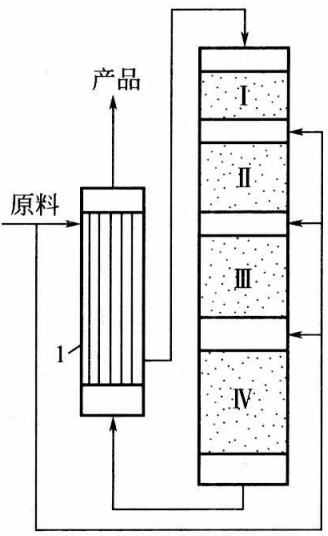
\includegraphics[width=.95\linewidth]{figures/fig7.3b.png}
        \end{minipage}

\end{frame}


\begin{frame}
    \frametitle{非原料气冷激式}

        \begin{minipage}{0.8\linewidth}
            \begin{itemize}
                \item 道理与原料气冷激式相同，只是采用的冷激剂不同。
                \item 所用冷激剂通常是原料气中的某一反应组分。
                \item[\bigcirc] 冷激式与间接换热式相比较，减少了换热器的数目。
                \item[\bigcirc] 此外，各段的温度调节比较简单灵活，只需控制冷气的补加量就可以了，流程相对简单。
                \item[\times] 缺点是催化剂用量较多。
                \item[\times] 非原料气冷激，是否有合适的冷激剂？
            \end{itemize}
        \end{minipage}\hfill
        \begin{minipage}{0.15\linewidth}
            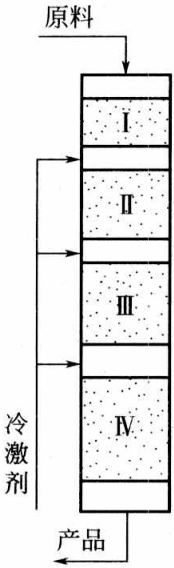
\includegraphics[width=\linewidth]{figures/fig7.3c.png}
        \end{minipage}

\end{frame}


\begin{frame}
    \frametitle{固定床绝热反应器的催化剂用量}
        \begin{minipage}{0.48\linewidth}
            物料衡算
    \[
        \frac{G w_{\mathrm{A} 0}}{M_{\mathrm{A}}} \times \frac{\mathrm{d} X_{\mathrm{A}}}{\mathrm{d} Z}=\eta_{0} \rho_{\mathrm{b}}(-\mathscr{R}_{\mathrm{A}})
    \]
        \end{minipage}\hfill
        \begin{minipage}{0.48\linewidth}
            热量衡算
    \[
        G C_{p t} \frac{\mathrm{d} T}{\mathrm{~d} Z}=\eta_{0} \rho_{\mathrm{b}}(-\mathscr{R}_{\mathrm{A}})(-\Delta H_{\mathrm{r}})_{\mathrm{T}}
    \]
        \end{minipage}
        \bigskip
    
    两式相除，得
    \[
        \frac{\mathrm{d} T}{\mathrm{~d} X_{\mathrm{A}}}=\frac{w_{\mathrm{A} 0}(-\Delta H_{\mathrm{r}})_{\mathrm{T}}}{M_{\mathrm{A}} C_{p \mathrm{t}}}
    \]
    积分之，
    \[
        T-T_{0}=\lambda X_{\mathrm{A}}
    \]
    \[
        \lambda=\frac{w_{\mathrm{A} 0}(-\Delta H_{\mathrm{r}})_{\mathrm{T}_{0}}}{M_{\mathrm{A}} C_{p \mathrm{t}}}
    \]
\end{frame}


\begin{frame}
    \frametitle{固定床绝热反应器的催化剂用量}

    积分物料衡算式，得
    \[
        L_{\mathrm{r}}=\frac{G w_{\mathrm{A} 0}}{M_{\mathrm{A}} \rho_{\mathrm{b}}} \int_{X_{\mathrm{A} 0}}^{X_{\mathrm{AL}}} \frac{\mathrm{d} X_{\mathrm{A}}}{\eta_{0}(X_{\mathrm{A}}, T)\left[-\mathscr{R}_{\mathrm{A}}(X_{\mathrm{A}}, T)\right]}
    \]
    两边分别乘以反应器横截面积，得催化剂体积为
    \[
        V_{\mathrm{r}}=\frac{F_{\mathrm{A} 0}}{\rho_{\mathrm{b}}} \int_{X_{\mathrm{A} 0}}^{X_{\mathrm{AL}}} \frac{\mathrm{d} X_{\mathrm{A}}}{\eta_{0}(X_{\mathrm{A}}, T)\left[-\mathscr{R}_{\mathrm{A}}(X_{\mathrm{A}}, T)\right]}
    \]
    无论是有效因子还是转化速率均随温度和反应物系组成而变，利用$T-T_{0}=\lambda X_{\mathrm{A}}$可把它们变成单变量$X_{\mathrm{A}}$的函数，便可进行积分。

\end{frame}


\begin{frame}
    \frametitle{}

    \begin{example}
        工业生产中的含酚废液及废气可用催化法将酚烧成二氧化碳和水，使其符合排放标准。现拟设计一固定床绝热反应器在0.1013 MPa下燃烧含酚气体中的苯酚。标准状态下含酚气体处理量为\SI{1200}{m^3/h}，苯酚摩尔分数为0.0008，于473 K下进入反应器，要求燃烧后气体中苯酚摩尔分数为0.0001。采用直径为8 nm以氧化铝为载体的氧化铜球形催化剂，在该催化剂上苯酚燃烧反应为一级不可逆反应，反应速率常数与温度的关系为
        \[
            k = 7.03 \times 10^6 \exp (-5000/T) \qquad \mathrm{min}^{-1}
        \]
        试计算催化剂用量（可忽略外扩散阻力）。
        
        数据：催化剂性质 \quad 比表面$= \SI{140}{m^2/g}$；颗粒密度$= \SI{0.9}{g/cm^3}$；
        
        \qquad 孔容$= \SI{0.42}{cm^3/g}$；曲节因子$=3$；床层空隙率$=0·38$。
        
        \qquad 反应气体的定压摩尔比热容为\SI{30}{J/(mol.K)}，反应热$=\SI{2990}{kJ/mol}$。
    \end{example}

\end{frame}


\begin{frame}
    \frametitle{多段绝热式固定床反应器}

    \begin{figure}[htpb]
        \centering
        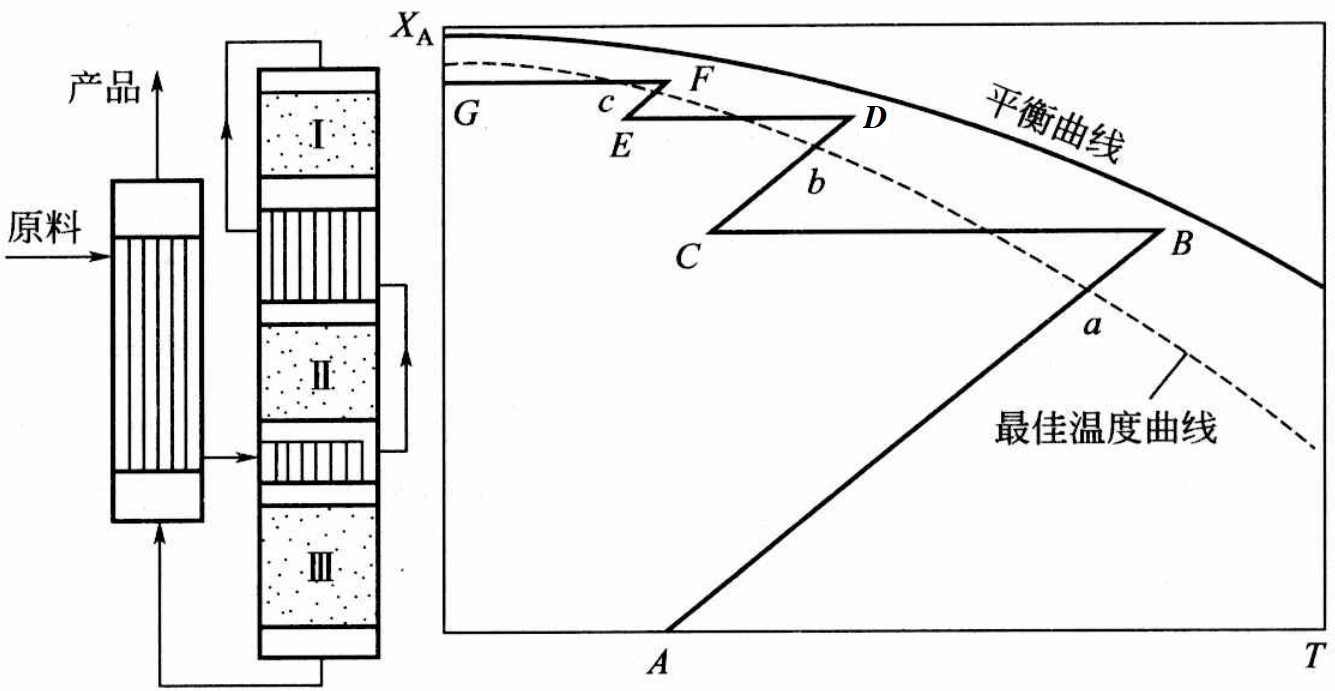
\includegraphics[width=.91\linewidth]{figures/fig7.4.png}
    \end{figure}

\end{frame}


\begin{frame}
    \frametitle{多段绝热式固定床反应器}

    以催化剂用量最少为目标进行优化，催化剂总用量为：
    \[
        V_{\mathrm{r}}=\sum_{i=1}^{N} V_{\mathrm{r} i}=V_{\min }
    \]
    为简化计，令$\eta_0 (X_{\mathrm{A}}, T)[-\mathscr{R}_{\mathrm{A}}(X_{\mathrm{A}}, T)] = \mathscr{R}_{\mathrm{A}}^{*}(X_{\mathrm{A}}, T)$，将单段催化剂用量$V_\mathrm{r}$的计算式代入上式有
    \[
        V_{\mathrm{r}}=\frac{F_{\mathrm{A} 0}}{\rho_{\mathrm{b}}}\left[\int_{X_{\mathrm{A} 1}}^{X_{\mathrm{A} 1}^{\prime}} \frac{\mathrm{d} X_{\mathrm{A}}}{\mathscr{R}_{\mathrm{A}}^{*}(X_{\mathrm{A}}, T)}+\int_{X_{\mathrm{A} 2}}^{X_{\mathrm{A2}}^{\prime}} \frac{\mathrm{d} X_{\mathrm{A}}}{\mathscr{R}_{\mathrm{A}}^{*}(X_{\mathrm{A}}, T)}+\cdots+\int_{X_{\mathrm{AN}}}^{X_{\mathrm{AN}}'} \frac{\mathrm{d} X_{\mathrm{A}}}{\mathscr{R}_{\mathrm{A}}^{*}(X_{\mathrm{A}}, T)}\right]
    \]
    
    

\end{frame}


\begin{frame}
    \frametitle{多段绝热式固定床反应器}

    
    \highlight 问 \bf{对于$N$段反应器，需确定的变量数目有多少个？}
    \bigskip

        \begin{minipage}{0.08\linewidth}
            
        \end{minipage}\hfill
        \begin{minipage}{0.88\linewidth}
            \begin{itemize}
                \item[$4N$] 各段进出口的温度及转化率共有$4N$个
                \item[$-2$] 最终转化率及进第一段的转化率已知
                \item[$-(N-1)$] 任一段的出口转化率等于下段的进口转化率
                \item[$-N$] 各段进出口的转化率和温度应符合绝热方程式
            \end{itemize}
        \end{minipage} 
        
    \[
        4N-2-(N-1)-N = 2N-1
    \]
    \highlight 答 \bf{需确定的变量数目有$2N-1$个}

\end{frame}


\begin{frame}
    \frametitle{多段绝热式固定床反应器}

    选择各段的进口温度$T_{i}$和除第一段外各段的进口转化率$X_{\mathrm{A} i}$作为控制变量，总数恰好也是$2N-1$个。
    
    将催化剂用量方程对$X_{\mathrm{A}i}$求偏导数，并令其等于零，得
    \[
        \mathscr{R}_{\mathrm{A}}^{*}(X_{\mathrm{A} i}, T_{i-1}^{\prime})=\mathscr{R}_{\mathrm{A}}^{*}(X_{\mathrm{A} i}, T_{i}) \qquad(i=2,3, \cdots, N)
    \]
    对$T_{\mathrm{i}}$求偏导数，并令其等于零，得
    \[
        \frac{\partial}{\partial T_{i}} \int_{X_{\mathrm{A} i}}^{X_{\mathrm{A} i+1}} \frac{\mathrm{d} X_{\mathrm{A}}}{\mathscr{R}_{\mathrm{A}}^{*}(X_{\mathrm{A}}, T)}=0 \qquad(i=1,2 \cdots, \mathrm{N})
    \]
    两式共包含$2N-1$个方程，求解此方程组即可确定各段进出口转化率和温度的最佳值。

\end{frame}
